\documentclass[12pt]{article}

\title{Approaches and Applications of Reverse Engineering}
\date{\vspace{-5ex}}
\author{Natalie Pargas}

\usepackage{graphicx}
\usepackage[left=1in,right=1in,top=1in,bottom=1in]{geometry}
\usepackage{amsmath}
\usepackage{hyperref}
\usepackage{setspace}
\usepackage{listings}

\spacing{1.5}

\begin{document}

\maketitle

% Latex can automatically build a table of contents for you
\tableofcontents
\newpage


\section{Introduction}
Reverse Engineering is the process of disassembling something in order to understand how it works. It has been done long before it was used for technology. For example, the dissections that were a common high school experience. They were done to break down something as mystifying as life into clear components and functionalities. One of the best ways to fully understand how something works is to open it up.

Reverse engineering software can be done in many ways. The methods of analysis can be divided into two categories, static and dynamic analysis. Static analysis involves combing over a snapshot of the code in a single state. Dynamic analysis is done when the program is being executed and changing states. To start reverse engineering, usually a program’s executable is passed to a disassembler which will break it down into the assembly level code. A programmer can use system monitoring tools to display information that was gathered by the operating system on the program and how it interacts with its environment. A debugger shows what happens in the CPU with the disassembled code one line at a time. Using these different tools, the programmer must use their intuition to guide the reversing process. 

There are many reasons why someone might want to reverse engineer software. The only time that the workings of software is available to anyone is when that software is open source. Open source software is freely available source code that anyone can view, share, and modify. However, software developers sometimes opt out of publicly distributing the source code. There are a number of potential causes for this, including licensing and ownership issues, the need to preserve proprietary data, or other personal reasons.

Some of the most common reasons a person would choose to reverse engineer software is so that they can perform malware analysis, improve programming skills, recover lost source code, and implement interoperability between programs. My first introduction to reverse engineering was through a video where the creator was reverse engineering Apple’s Facetime for Mac so he could reinstate closed captioning for his hearing impaired mother. The list of uses is as extensive as programs out there.

 Most software developers know reverse engineering in the context of malware analysis. A classic example is a Trojan virus. Malicious developers can hide malware in programs that are designed to look innocuous. Breaking apart these programs will unveil the malware hidden inside. Developers also often call on external libraries. With large projects, keeping track of dependencies can be hard. Hackers can hide entry points in these libraries so they can access unauthorized information. Reverse engineering is the only foolproof way to reveal exactly what is happening at each step of a program’s execution.

Learning how something is being done can be great to improve skills. Reverse engineering requires extensive knowledge of both assembly code and how high level code structuring. Reverse engineering someone else's code is no simple feat and will cause the reverser to need to learn in depth the possible ways a program could be constructed. This project will be an endeavor in learning both forward engineering and reverse engineering.  

People may reverse engineer their own program to recover lost source code. While this is no easy task, it is possible to use reverse engineering to recover source code. Many software developers know the pain of losing source code and, with an executable, reverse engineering offers a potential solution.

Interoperability is one of the reasons a person might choose to reverse engineer something. This purpose is also only able to be accomplished through reverse engineering. When working with external libraries or operating systems that have documentation on usage but no source code, oftentimes documentation doesn’t cover all use cases. While a programmer could keep throwing things at the wall or try to contact the vendor, reverse engineering provides a surefire way of figuring things out.

For this project, the goal of reverse engineering is to grow my knowledge of reverse engineering specifically in the context of mobile applications. I will do that by designing an RGB slider Swift app and then reverse engineering it to try and see if I can identify all of my source code. Further goals with this project are to achieve interoperability with an existing makeup app so I can inject my own functionality.

\section{Analysis Methods and Tools}
\subsection{Static Analysis}

Static analysis is a practice of analyzing code without executing it. It can  be used to help inform dynamic analysis. Static analysis tools can analyze at either the source code level with code that hasn’t been compiled yet or machine language level with code that has. Static analysis tools can be used by reverse engineers to retrieve and comb over assembly level code. This is one of the most basic functions of any static analysis tool, but many of them offer a lot more functionality to help reverse engineers. Most static analysis tools are designed to help give the reverse engineer a starting off point with interpreting assembly level functions.

\subsubsection{Disassembler}
One of the most key static analysis tools for a reverse engineer is a disassembler. Disassemblers are applications that take in a program’s executable file and generate a file with the assembly code. This isn’t too difficult because assembly is just a text translation of the machine readable binary code. Unfortunately, that makes it a lot less clear than higher level programming languages.  Disassembly is also unique to a person’s processor, but there are disassemblers that can support more than one CPU architecture. Some examples of disassemblers are IDA, Binary Ninja, Hopper, Ollydbug, Radare2, and Ghidra (what I’ll be using for this project). 

\subsubsection{Decompiler}
Decompilers are similar but more complex than disassemblers. Instead of just producing the assembly language code, decompilers attempt to produce high-level readable code. They attempt to produce something that looks as close to the source code as possible by reversing the compilation process~\cite{Reversing}. The front end of the decompiler decodes low-level assembly instructions and translates it into an intermediate representation specific to the decompiler. The intermediate representation is then iterated on to remove as many extraneous details as possible while preserving the important details. Lastly the back end takes the polished up intermediate representation and translates it again into a high level language.

While this may sound like a simple way to retrieve the source code, it is highly unlikely the high level language returned will be something that actually matches. Anyone who has ever run text through a translation website multiple times knows that each iteration causes a loss in fidelity and oftentimes the end result will be gibberish. Decompilers go a step further and have no immediate knowledge of things like function or variable names and structures. This does not make them useless, though. For example, a text translator will usually return your original result when given a simple phrase. Similarly a decompiler will most likely be able to pick up on more straightforward functions such as adding a + b. Decompilers offer hints and snippets into what the source code may look like which is valuable information for a reverse engineer. Most of the examples for disassemblers listed also count as decompilers.


\subsubsection{Dumping Tools}
Executable dumping is usually the first step in reverse engineering a program. Executable dumping helps inform a reverse engineer what a program does, how it interacts with external elements, and general knowledge of how a file is structured. Using dumping tools, a reverse engineer will start by figuring out what type of file they’re dealing with. They will then start to unpack the format. Extracting strings will immediately offer insight into what language the source code is written in, what library modules it uses, what kinds of data it is dealing with, and what the goals of program functions may be. Other useful information we can retrieve is the layout of the file in memory and what the general logical structure of the file is. Once we know the type of file we also know which tools we can use. For example, some debuggers only work with certain high and low level languages. Some popular executable dumping programs are ones already built into your machine like DUMPBIN for windows or otool for mac. 
Otool is especially necessary for this project because it identifies a file's mach header. On systems with a Mach kernel like macOS and iOS, the executable binaries they use will have a mach header. All headers have a magic number to identify them. Thin binaries only have that number while fat binaries with fat headers will have locations of the other executable's headers in them ~\cite{mobileRe}.


\subsection{Dynamic Analysis}
Dynamic Analysis occurs when the program or section being analyzed is run during the analysis process. Because dynamic analysis requires the program to execute with unknown results, it is safest to do it in an enclosed or sandboxed environment to protect the rest of the system~\cite{MasteringRE}. Thus easily manipulated virtual machines are usually set up during the dynamic analysis process. Many tools can be part of the dynamic analysis process. Anything that needs to run and monitor some output is considered dynamic. Tools may run the full program, a portion of the program, or even just a single line. Tools that monitor the external environment while the program runs are also considered dynamic.

\subsubsection{Debugger}
Debuggers are a tool usually used for developers to locate and work through errors in their programs, but they’re also vital tools in reverse engineering. Many debuggers can work through assembly language. While assembly language may be difficult for a human to parse through, it is the exact same logic that gets broken down and sent to a computer meaning that the computer can show what each assembly instruction is intended to do. Most debuggers software engineers use were actually designed from the ground up with the purpose of stepping through assembly code. The debugger can show the state of CPU registers along with a memory dump that shows what’s in the stack~\cite{Reversing}. Debuggers usually contain disassemblers which as discussed is a vital reverse engineering tool. Many debuggers also contain both software and hardware breakpoints. Software breakpoints are instructions added into the code during runtime to pause and hand control over to the debugger. Hardware breakpoints are a CPU feature which allow the processor to pause execution when a certain memory address is reached and hand control over to the debugger. A reverse engineer can use insert breakpoints at data structures of interest and use the debugger to reveal what they are. Debuggers also offer a clear view of registers and memory to aid in a reverse engineer's ability to process low level information.

\paragraph{\underline{User Mode Debuggers}}
Most debuggers that a programmer will use are user mode debuggers. They run on a system like any other application then seize control of the target program to debug ~\cite{Reversing}. An advantage to them is that they are easier to set up and navigate than their kernel-mode counterparts. Usually it’s fine to stay limited to user mode viewing of an application. It only creates troublesome limitations when the target application has kernel mode components such as device drivers. User mode debuggers are also not always sufficient when trying to debug a program before it reaches the main entry point. These kinds of programs are usually ones that have a lot of statically linked libraries in the executable. The final and most likely to be problematic issue is that user-mode debuggers can only view a single process in a program. This can cause issues when the target application has processes that interact in unknown ways. The user may not know which process to zero in on that has the code of interest.

\paragraph{\underline{Kernel Mode Debuggers}}
Kernel mode debuggers are different from user-mode debuggers because they capture the entire system and not just a single process. Instead of running atop the operating system, kernel mode debuggers sit alongside the system kernel and stay ready to capture the entire system’s stats. Kernel mode debuggers can be more helpful to reverse engineers because they offer more clues as to what’s going on with the system. A key tool for kernel-mode debuggers is that they allow the placement of low level code breakpoints. As a reverse engineer working with assembly code, being able to test different sets of assembly instructions that may be the code section a reverser is looking for is incredibly useful.

For example, picture a scenario where a reverse engineer is looking for the API responsible for handling moving windows? That will need to be managed by a windows manager in the kernel. The complexity is introduced when trying to identify which API moves a particular window. Since there are multiple APIs that can be used to move a window, pinpointing the one you are trying to focus on is a difficult task. This is where kernel mode debuggers come in handy. Low level breakpoints in the operating system responsible for shifting windows around will help you identify which API is getting called when a window is moved~\cite{Reversing}. From there the reverse engineer will be able to hone in on that API.
Unfortunately, kernel mode debuggers come with their own drawbacks. Setting them up can be challenging because they require access to the full system. They need to suspend the entire system while running so they can go line by line, which means the system can no longer have multiple threads going~\cite{Reversing}. They will also usually need to be set up inside a Virtual Machine which will be discussed in a later section~\cite{PracticalRE}. These are reasons why a reverser should exhaust their other options before jumping into using a kernel mode debugger. Still, they are powerful tools when the scenario calls for it.

\subsubsection{System Monitor}
System monitoring can be a crucial part of the reverse engineering process. In some cases, a reverse engineer can figure out what they need through system monitoring tools without ever looking at the decompiled code. System monitoring tools can capture what happens between the code and hardware using the intermediate channels of input/output~\cite{Reversing}. For local system monitoring, tools monitor things such as file operations (creating, deleting, moving, etc). For programs that communicate over networks, system monitoring might look like recording all TCP/UDP network traffic. System monitoring tools are commonly used in virtual machines.

\subsubsection{Virtual Machine}
Many programmers will encounter virtual machines (VM) at some point during their career. It’s not uncommon for an application to interface exclusively with one type of operating system. One reason is because writing applications to work with different operating systems adds time and complexity that not all programmers can afford. Choosing to write in a high level language may make code more portable because there’s more verbose built-in libraries or interpreters that deal with the specifics of the systems without the need for any programmer intervention. But high level languages often trade performance for convenience which is not a trade that a developer working with large amounts of data can necessarily afford to take.
What happens when a developer has an application that runs on Windows while they have a Mac? This is where a virtual machine enters into the mix. Virtual machines are safe sandboxed environments that work as miniature computers with their own operating systems within a computer. They are constructed with an interpreter and bytecode. During compile time, select code snippets are compiled specific for the VM target architecture and then inserted into the program along with the interpreter. During run-time, the interpreter begins executing the bytecode. Virtual machines are costly to implement because they are so expansive which is why only the necessary code snippets get rendered~\cite{MasteringRE}.
Because virtual machines work in their own isolated environment, they offer powerful protections against unknown or potentially malicious software. This makes them a useful tool for reverse engineers who deal with software that they do not know the contents of. The level of control over virtual machines also makes them a useful tool because there is ultimate knowledge of system conditions.


\section{Understanding Program Structure}
It is important for a reverser to understand the different goals of high level and low level languages. Understanding these differences will help with interpretation of why code is structured a certain way.


\subsection{High Level Languages}
High level languages exist to take away the complexity of system specific programming. High level languages work so that a programmer can focus on specifying the clean structural logic without needing to dedicate time to figuring out system specific details. While writing in something like assembly can be very performative, it would be nearly impossible for a standalone human to write a modern application in assembly.
Because high level languages favor simplicity over the flexibility to do exactly what is the most efficient for achieving a program’s goals, many programmers don’t even know what is going on at the assembly level. A reverse engineer will be forced to pick apart what potentially roundabout ways a program’s goals are being achieved. The main goal of a reverse engineer is to use what they know about what the program was trying to do, potential ways that can be accomplished in high level code, and how to read assembly code to make their best educated guess on what’s happening where.
For reverse engineers, the most important thing to know about a high level language is to what level does it abstract or conceal the underlying machine code~\cite{Reversing}. Languages like Python that have a built in interpreter will abstract it a lot. These programs may be full of extraneous machine code. On the other hand, languages like C are written much closer to the target processor and won’t have nearly as much separation between the source and machine code.

\subsubsection{Control Flow}
The name of when languages simplify minute details for the programmer is ‘control flow’. Control flow is what makes code more user friendly. This manifests through statements like conditionals that give general instructions for what a program should do when. A processor has no knowledge what statements like ‘if’ or ‘while’ mean. Under the hood, these statements translate into verbose and daunting assembly code. This is because high level conditional statements are often broken down into operation sequences because it would otherwise overwhelm the processor~\cite{Reversing}.

Other typical structural components of programs that aid in control flow are switch blocks and loops. Switch blocks, or \(n-way\) conditionals, take in an input and have \(n\) number of code blocks that are potentially executed depending on the input value. Each block of code gets assigned at least one value prior to runtime. The compiler also generates code to receive the input value and search for the proper code block to execute. The values for the code blocks are usually stored in a lookup table that has pointers to each corresponding code block.  Depending on the input value, the program will go through the process of searching the lookup table then jumping to the proper code block at runtime~\cite{Reversing}. Loops work to allow a program to repeatedly execute a certain code block multiple times. A loop has a counter to keep track of how many iterations it has performed. There is also a conditional statement that determines when the loop will stop. Loops and conditionals are inherently intertwined. The difference is that loops execute over and over until the condition is no longer met.

To understand control flow sequences, one must understand how low level control flow is implemented. This means that a reverse engineer needs to know the specific rules of each kind of low level architecture because low level control flow is individual to the platform and therefore the language.

\subsection{Low Level Languages}
Earlier we mentioned that complexity is introduced when working with low level system specific details. This is especially true when the goal is to translate high level logic into something that will be understood by your machine. Of course, there must be a way to do this because the CPU does it anytime a modern application is run. But it often involves keeping track of more details than a sole human is capable of. That is why a reverse engineer must develop the skill of parsing through assembly code and being able to create a kind of ‘mental image’ of how it relates to high level constructs.
Data management is one of the things that a person’s computer keeps track of that would be difficult for a human to do. To understand why this is, we can look at the data management of a relatively low level language, C, versus the assembly representation. Consider the code: 
\begin{lstlisting}

int divide(int a, int b) {
    int result;
    result = a // b;
    return result;
}
\end{lstlisting}
While this function may seem incredibly simple, there is no direct translation into a machine code representation. To execute this in a low level language, it would require first storing the machine state. Then memory would need to get allocated for result. Variables a and b would need to get loaded from memory into a register. Then a would need to be divided by b and the result would need to get stored in the register that got loaded in the beginning. The machine state from before would need to get reloaded. The pointer would need to return to the caller and bring back result~\cite{Reversing}.
One line of high level code could result in any number of assembly instructions. Managing data is one of the biggest challenges of reverse engineering.

\subsubsection{Registers}
To keep from needing to constantly access RAM, microprocessors have a smaller internal memory that can be accessed with barely any performance cost~\cite{Reversing}. There are multiple types of internal memories that microprocessors keep and registers are one of them. Registers are little pieces of internal memory that live within the processor and are able to be accessed with an imperceptible cost to performance~\cite{PracticalRE}.
The biggest problem with registers is that there are not very many of them. One of the most popular processors, the IA-32, only has eight 32-bit registers that can be used for anything. It does have more registers, but they all have highly specific use cases. Assembly language is written around utilizing registers because they’re so performant. They are not good for long term storage, though, that is when RAM becomes the better choice. One of the most important things to take away is that CPUs do not automatically manage this. Data management is outlined in the assembly code which is what reverse engineers will need to get comfortable sorting through.
One thing that reverse engineers will need to do is focus on figuring out what kind of values are getting loaded into a register. For example, it is easy to see when a register is only being used to grant instructions access to a specific value because that register will only show up when transferring value from memory to the instruction or vice versa. Another example is when a register shows up many times in one function. This is a good clue that one of the function's local variables is being stored in that register.
\begin{figure}[h]
    \caption{Figure modified using Intel® 64 and IA-32 Architectures Software Developer’s Manual and https://flint.cs.yale.edu/cs422/doc/pc-arch.html\#register}
    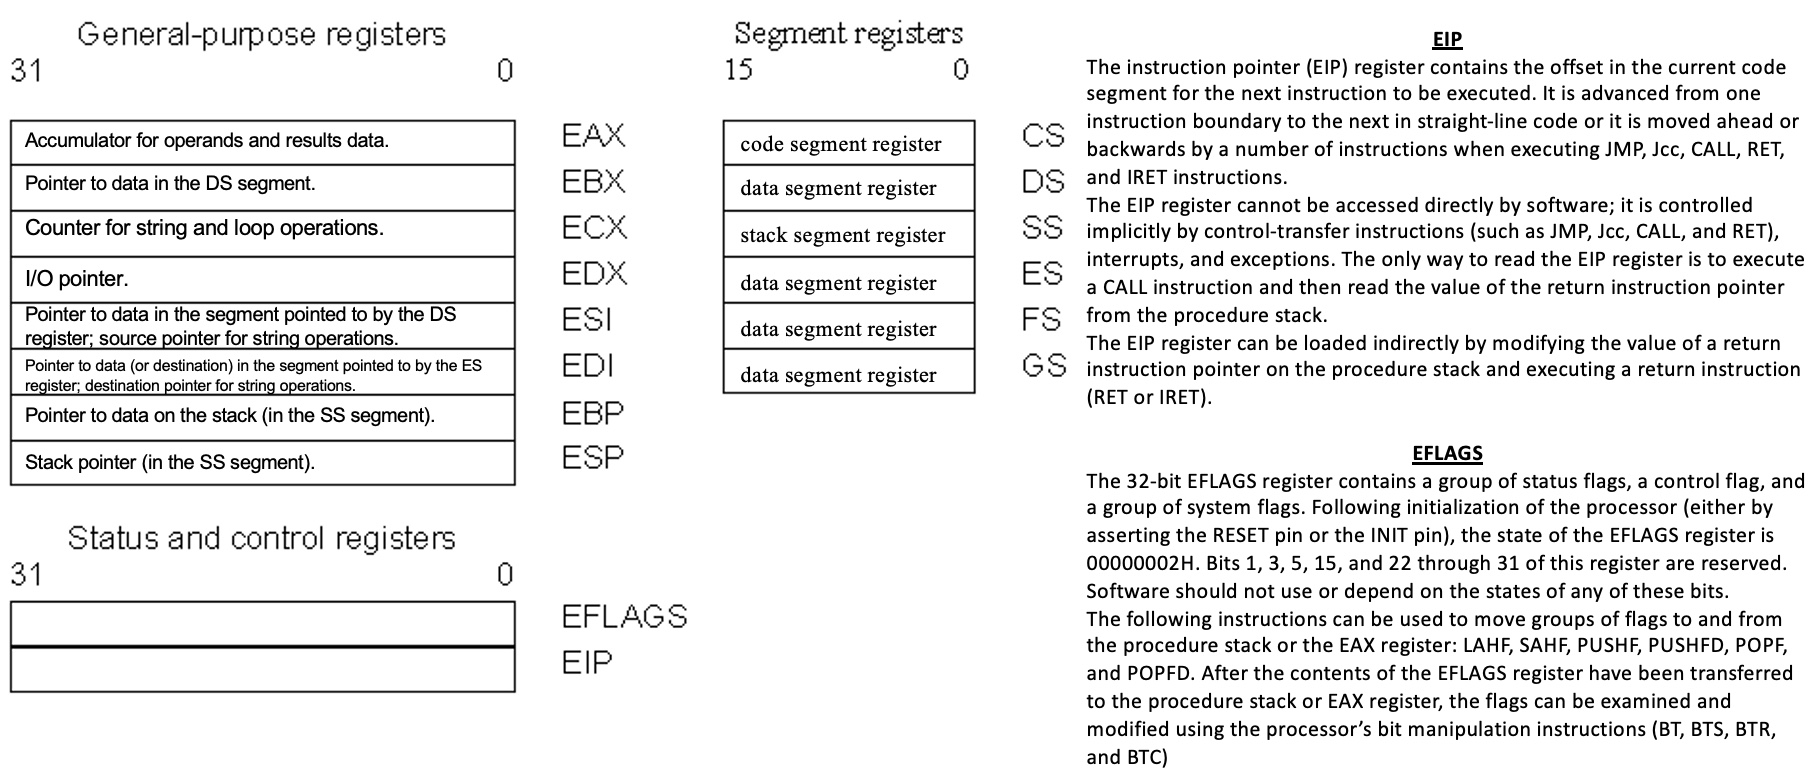
\includegraphics[scale=.27]{Junior IS/Register Diagram.jpeg}
\end{figure}

\subsubsection{The Stack}
The stack is one of two places that a value can be set aside. Registers are not managed by a processor and to use one you just need to load a value in it. Often there will not be registers available or there is a particular reason a variable will need to reside in RAM instead of in a register. That’s when you’d put a variable on the stack instead~\cite{Reversing}.

The stack is a short term storage space in memory that gets utilized by both the CPU and the program. It is the spot where short term information gets put when a register can not be used for whatever reason. Registers are for the shortest term data while the stack is for the second shortest. The stack lives in RAM like all other data and is just a carved out section for intermediate term data. Modern operating systems tend to manage multiple stacks at the same time. Each of the concurrently running stacks is a representation of a program or thread~\cite{MasteringRE}.

Stacks use Last In First Out data management. Items are pushed on the top of the stack and popped from the bottom of the stack. Memory in stacks is allocated from the top down where the first in address is allocated and used first while the stack grows backwards towards lower addresses~\cite{Reversing}.

\subsubsection{Flags}
One of the registers you may have noticed from the previous figure is the EFLAGS register. This is a collection of special IA-32 registers that contain system and status flags. The system flags’ job is to manage the different modes and states of the processor. The status flags are what a reverse engineer will typically be more interested in and are used by the processor to record its current logical state~\cite{Reversing}. They are often updated by various logical and integer instructions so they can record the outcome of these actions. There are also instructions whose operation conditions are dependent on the values for the status flags. This is what allows sequences of instructions to run different operations depending on what different input values may be, etc. 

Flags in IA-32 are the crux of conditional code. Arithmetic instructions check operand conditions and then set processor flag conditions based on the resulting values. There are also sets of instructions designed to read the flags and do different operations based on the value. An example of a popular instruction set is Jcc or the Conditional Jump. It tests for predefined flag values and then jump depending on whether or not it matches with the specified conditional code~\cite{intelManual}.

\subsubsection{Instructions}
Instructions are the actual actions specified in assembly code. They are formatted with operation code (opcode) and one or two operands~\cite{Reversing} The opcode is what you are asking the computer to do such as MOV or JMP. The operand is the parameters that get passed to the opcode or the data being manipulated. Certain instructions will have no parameters. Data in assembly comes in three basic forms. There are register names, immediate data, and memory addresses. Register names are the names of the general purpose registers to be read from or written to like the EAX, EBX, etc. Immediate data is constant values that are embedded into the code and usually indicates there was a hard coded value in the source code. Memory addresses are the locations of operands stored in RAM. It can be hard coded and tell the processor where to read to and write from. It could also be a register with a value that will be used as a memory address. It is also possible to combine a register with an arithmetic operation and a constant so that there is some base address and then an index offset~\cite{Reversing}.

General purpose instructions are the ones that deal with program flow, logic, arithmetic, string operations, and basic data movement. They deal with data stored in memory at the general purpose registers, EFLAGS register, segment registers, and address information stored in memory ~\cite{Reversing}.

The MOV instruction shows up most frequently in most IA-32 instruction sets. This one deals with basic data movement. It takes in a destination operand and a source operand then moves the data from the source to the destination. The sources can be registers, immediate, or memory addresses. It is important to note that MOV cannot transfer data through memory, it can only take it out or put it in. The destination address can be a memory address (using a register or an immediate) or a register~\cite{Reversing}.


\section{Implementations}

\subsection{Reversing Hello World}
Before taking on the larger endeavor of reversing a program written in a declarative language (SwiftUI), it’s important to start with the basics. Figure [insert figure here] shows a simple ‘Hello World’ program in C. To add some complexity, a few random variables and data structures were thrown in as Easter eggs. This is the program whose decompilation will be used as a jumping off point.
\begin{figure}[h]
\caption{Hello World Program}
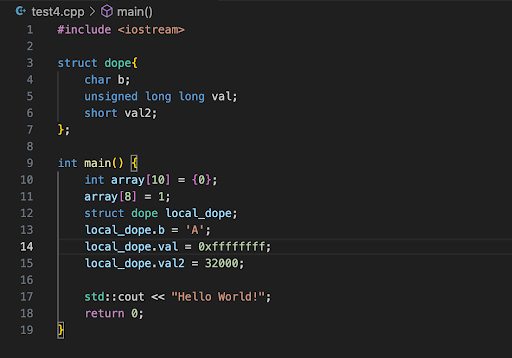
\includegraphics[scale=.75]{Junior IS/HelloWorldSource.png}
\end{figure}
Figure 3 is the decompilation of the program once it was put through Ghidra. The first thing to note is how with even a relatively low level language like C, the instructions in the code more than doubled. The disassembly being shown in the figure is also only a portion of Ghidra’s output. The figure only shows the function section of the program output when imports, exports, labels, classes, etc take up the large majority of the program. One important part of reverse engineering is sorting through all of the information to find out what exactly is important to the reverser. Some reverse engineers refer to this process as finding the shape and edges of the data. 
\begin{figure}[h]
\caption{Hello World Disassembly}
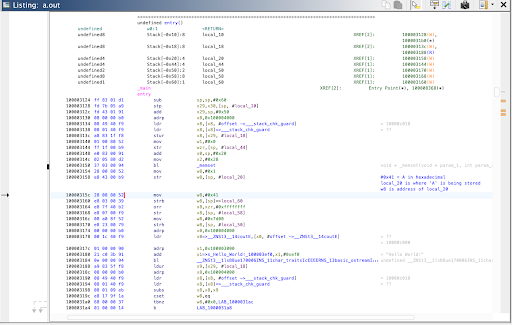
\includegraphics{Junior IS/HelloWorldGhidra.png}
\end{figure}
With the important section identified, it is time to analyze the assembly code. One thing to keep in mind with the disassembled code is that all the values will be stored in hexadecimal. A good place to start is with the values we know will need to be stored. In the array there are 10 variables which all get set to 0, except for the eighth array member which is changed to equal 1. In our local\_dope struct there are three variables equal to ‘A’, ‘0xffffffff’, and 32000. The highlighted line in the figure shows ‘A’ being stored in the register w8. Shortly after, \#0xfffffff shows up without needing to be translated into hexadecimal. \#0x7d000 is the hex for 32000. This surface level analysis offers a glimpse into the methodology of more complex reverse engineering. Lastly, the 'Hello\_World!' gives us the final piece of information we need to know about what the program is.


\subsection{Crack Me Problems}

The next step in practicing reverse engineering is trying a Crack Me problem. Crack Me problems are toy problems designed by other software developers to help reverser's practice their skills. Usually there’s an executable that opens up a little puzzle. The puzzles usually involve finding a password but can involve any number of things like decryption, key generation, etc . This section will cover the process of reverse engineering a simple crack me.

The first step I took in reversing this program was checking the header and libraries as shown in Figure 4 and 5.

\begin{figure}[h]
\caption{Crack Me Header}
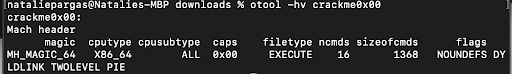
\includegraphics{Junior IS/crackmeheader.png}
\end{figure}
\begin{figure}[h]
\caption{Crack Me Libraries}
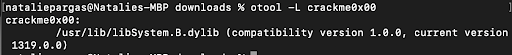
\includegraphics{Junior IS/crackmelibs.png}
\end{figure}

Both of these steps were done with an executable dumping tool called ‘otool’. The header information shows that the assembly language being used is x86. The library dump shows that the only library being linked is the system library. While these tools didn’t offer that much information about this particular program, they are very useful in programs that have more dependencies and more specific assembly languages. These dumping tools ended up being vital later in the project because they offered insight into what libraries were being linked from the project's declarative language as well as what assembly language was being used with Apple’s modified version of ARM64. Next, otool was used once again to list the strings. This is a vital part of reverse engineering and is useful to be able to refer back to during the process. Figure 6 shows the result of the string dump.


\begin{figure}[h]
\caption{Crack Me Strings}
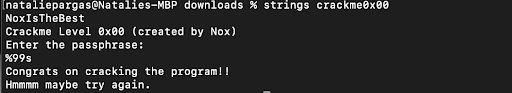
\includegraphics{Junior IS/crackmestrings.png}
\end{figure}

Examining this more closely, you can see that there’s only a few strings that give a very clear idea of what the program is designed to do. There’s a random string, the title of the program, a passphrase prompt, a string indicating the expected input, a congratulations message, and an incorrect guess message. With just this information, you could easily make an educated guess on what the password is. Most likely the passphrase will be the one random string that doesn’t get given easily in the executable. But for the sake of gaining understanding of the process, it’s good to go over the decompiled code. Figure 7 shows the decompiled code.

\begin{figure}[h]
\caption{Crack Me Ghidra Disassembly}
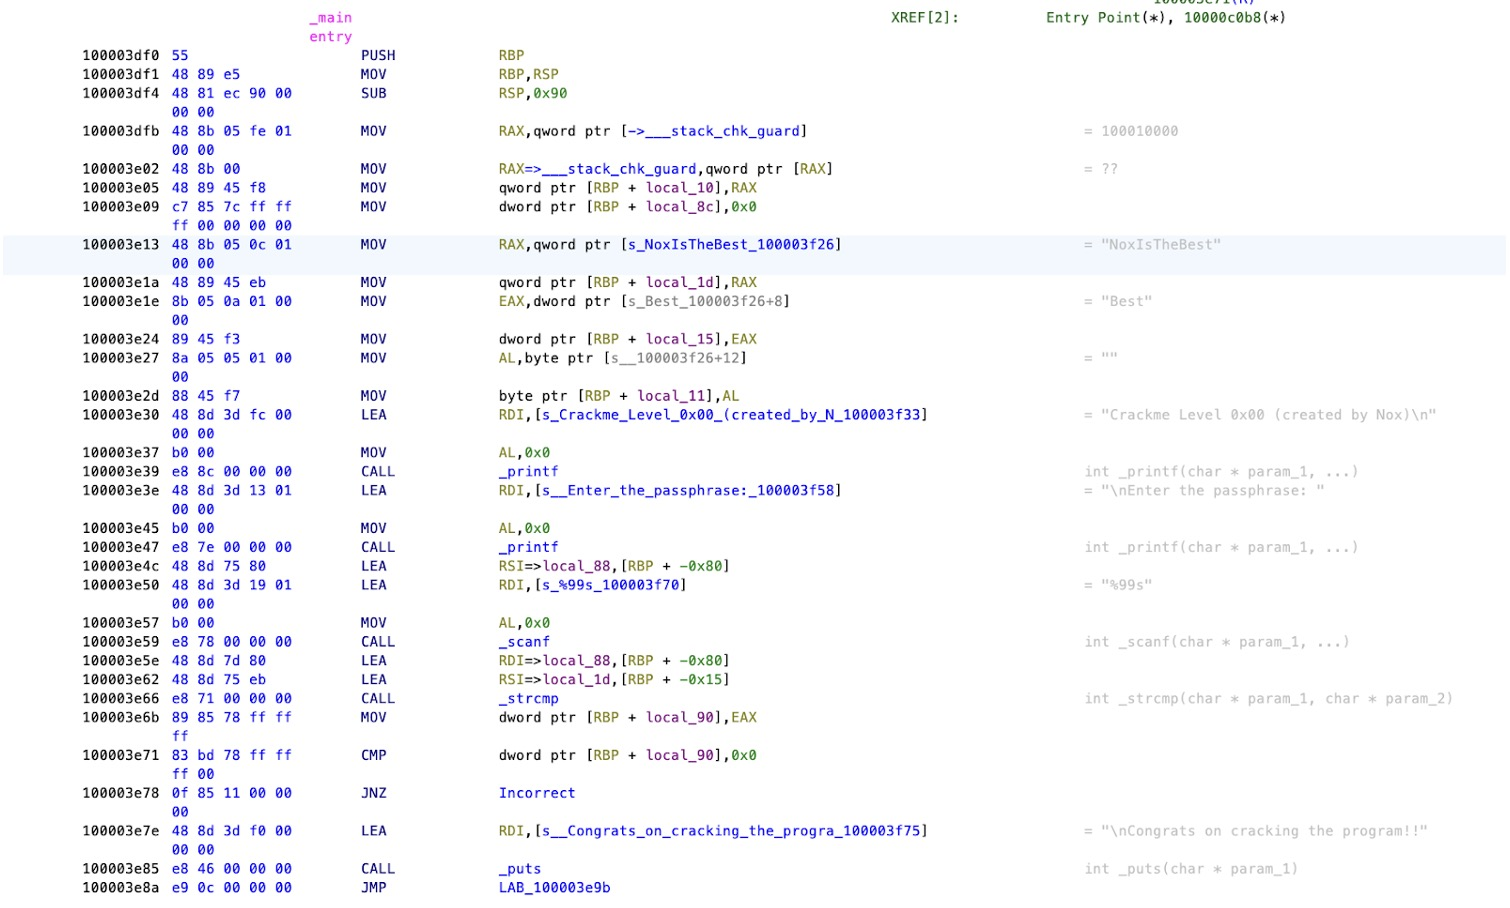
\includegraphics{Junior IS/crackmeghidra.png}
\end{figure}

The first thing to do is find the entrance into the program. Ghidra already labeled the ‘\_main’ at the top but the strings and function calls reaffirm this as the right section to be looking over. Next, thinking back to the string dump, it’s likely that the password will be near whatever function takes input. Prior knowledge of programming informs the reverser that after getting the user input, the input string will need to be compared to the right answer. Thankfully Ghidra was able to identify the function ‘scanf’.

\begin{figure}[h]
\caption{Crack Me Code Section 1}
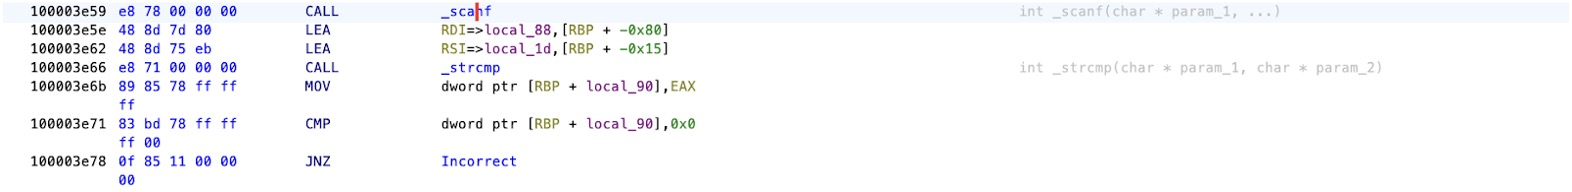
\includegraphics{Junior IS/crackmescanf.png}
\end{figure}

Inspecting the code section at figure 8, it shows that the variable local\_88 contains the user input. This is because it loads a \%99s into the RDI register to prepare for the input directly above where scanf is called. RSI has local\_1d loaded into it and that variable is immediately ‘strcmp’ compared to local\_88. Using these clues, one could infer that local\_1d contains the password. To verify, a reverser should always retrace and check.

\begin{figure}[h]
\caption{Crack Me Code Section 2}

\includegraphics{Junior IS/crackmeRAX.png}
\end{figure}

The first instance of local\_1d contains the register RAX 9. RAX has the qword ptr ‘ s\_NoxIsTheBest\_100003f26’ moved into it right above. s\_NoxIsTheBest\_100003f25 only contains the string “NoxIsTheBest”. That string is probably the password, but all that’s left is to check. Figure 10 shows the result.
\clearpage
\begin{figure}[h!]
\caption{Crack Me Code Executable}
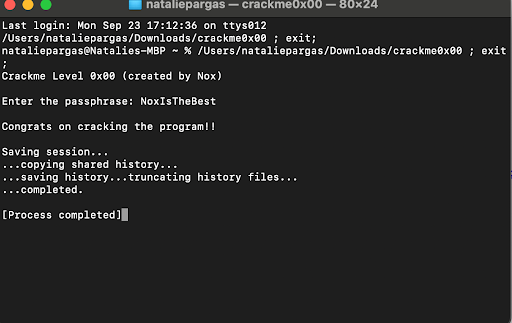
\includegraphics[]{Junior IS/crackmeexe.png}
\end{figure}
The attempt was a success and the crack me was successfully reverse engineered!


\subsection{Making An App}
The next endeavor for this project is creating an app in Swift. iOS apps are usually built using a combination of Swift, Objective-C, and Swift UI. Objective-C methods are stored using dynamic function pointers that get resolved at runtime. The names are intact in the binary so they’re easy to find when disassembled ~\cite{mobileRe}. An iOS app contains an info.plist file, an executable, and resource files. The info.plist file has key-value pairs in it that are necessary for runtime-configuration. The executable is the local file to run that contains the entrypoint and statically linked code. Resource files are the files required by the application to properly run ~\cite{mobileRe}. Figure 11 shows the breakdown of an ios app.
\begin{figure}[hbt!]
\caption{iOS Application Layers}
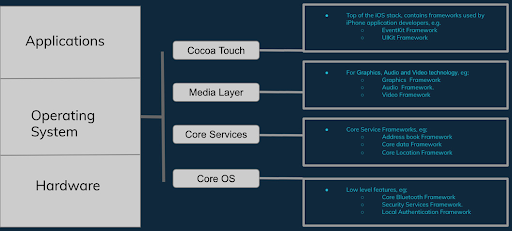
\includegraphics{Junior IS/ioslayers.png}
\end{figure}
The goal for this project was to create an RGB slider. This ended up being a task that could be done with mostly SwiftUI code. That means a lot of the coding was done in the Cocoa Touch layer. One of the key differences between SwiftUI and other languages is that it uses views instead of classes. This will be very important when getting into the disassembled code. But, it was relatively straightforward when working through one of their tutorials. Figure 12 shows the combination of their first two tutorials on using views.
\begin{figure}[h!]
\caption{Apple Swift Views Tutorial}
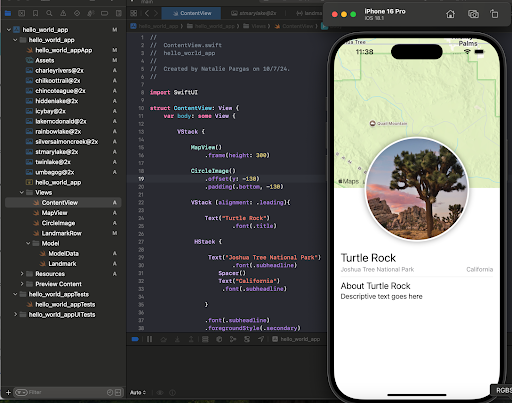
\includegraphics[scale=.75]{Junior IS/swiftuiviews.png}
\end{figure}
This project’s app only needed one view because of the simplicity. Figure 13 shows the app.
\begin{figure}[h!]
\caption{Crack Me Code Executable}
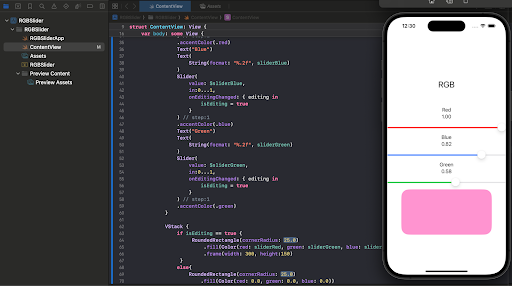
\includegraphics{Junior IS/appsc.png}
\end{figure}
The sliders control the amount of each color going into the rectangle. Whenever a slider is edited, the result gets passed back to the \_isEditing variable and the rectangle updates the color value. The next step is to reverse engineer this app.

\clearpage
\subsection{Reversing An App}
The final goal of this project is to reverse engineer the RGB app now that it’s been forward engineered. Having the source code available during this process was absolutely vital because it ended up being more complex than expected. The obvious clues that were available in the crack me problem like clear strings or function names were obfuscated in Apple’s SwiftUI disassembled code. Because of the complexity, the in depth analysis is provided in a separate document.  

There were a few key findings during the reverse engineering process. The first thing I discovered was that all of the text I input in the program was encrypted. This wouldn’t have necessarily been the case had I used a different method for printing text. Apple has both ‘Text()’ and ‘String()’ functions. The Text() function is the one that’s used more predominantly and automatically assigns ownership of the enclosed text to the stack it’s wrapped in as well as encrypts the text. The function names in SwiftUI also are automatically mangled and must go through a name unmangling algorithm at runtime which is provided by a separate DLL. One of my most major discoveries was the way SwiftUI’s views were handled by the assembler. Views are treated as both functions and labels depending on the context. Vertical Stacks and Horizontal Stacks (wrappers designed to orient objects on a page) were also handled differently depending on the context. Another surprising finding was how instructions were allocated for performance. There were a few instructions such as ‘adrp’ that were less common assembly instructions but still showed up frequently in the disassembled code. After performing this operation by hand multiple times, it became apparent that it was used almost exclusively to zero out a register instead of manually moving data around. Most likely this is because it’s faster for the CPU to perform this instruction instead of loading and moving data. Another thing to keep in mind when looking over the analysis is the alterations Apple made on regular ARM64. Certain registers like x18 are reserved, byte alignment may not be exact, different data types may be signed differently, etc. The documentation outlining all the differences can be found here: \url{https://developer.apple.com/documentation/xcode/writing-arm64-code-for-apple-platforms}. 
Another reason why reverse engineering is challenging is because the process of building an executable is destructive so you have to use your own inferencing abilities to guess what the source code is. 


\section{Conclusion}
As a beginner reverser, taking on the task of reversing a highly abstract language with multiple layers of security was very challenging. As languages continue to grow, as do the layers of abstraction from machine code. SwiftUI was approximately as high level as it gets so there were a lot of layers to traverse through. 
Reverse engineering is also a process that can be as complex or shallow as an individual chooses to make it. There was even more freedom with how specific the analysis should be because the source code was readily available. Despite this, even the process of solidly pinpointing where the self written code was a weeks long endeavor. Because reverse engineering is more of an individual art than a formulaic process, there is limited formal literature available on it. The academic literature that does exist also quickly becomes outdated as new languages and operating systems arise. For example, much of this paper was written with 32-bit architecture as the subject while 64-bit architecture is actually much more prevalent now. Unfortunately, the literature on reversing 64-bit architecture is mostly limited to documentation or blogs.
Having the source code available ended up being necessary to my project to combat the destructive nature of building an executable. With any build process, fidelity is lost during the translation of source code to assembly. There is also a many to many relationship between source and assembly code where the source code for an application can have \(n\) number of assembly representations. Documentation of Apple’s framework libraries was not always available to be able to trace where or why some piece of assembly was generated. Having the source code be readily available was the only reason this project was possible. 
Ultimately, there is a lot of potential in the space of researching reverse engineering as a whole. 


% Bibliographys
\pagebreak
\nocite{*}
\bibliographystyle{plain-annote}
\bibliography{bibliography.bib}

\end{document}